\documentclass[10pt]{article}
\usepackage{amsmath,textcomp,amssymb,geometry,graphicx,enumerate,tikz,algorithm,algpseudocode,pifont}
\usetikzlibrary{calc}
\usetikzlibrary{datavisualization}
\usetikzlibrary{datavisualization.formats.functions}


\textheight=9in
\textwidth=7in
\topmargin=-.75in
\oddsidemargin=-0.25in
\evensidemargin=-0.25in

\usepackage{listings}
\lstnewenvironment{codeblock}
    {\lstset{language=Python,
      showspaces=false,
      showtabs=false,
      breaklines=true,
      mathescape=true,
      showstringspaces=false,
      breakatwhitespace=true,
      commentstyle=\textit,
      keywordstyle=\textbf,
      basicstyle=\ttfamily,
      escapechar=`,
      moredelim={**[is][{\color{RoyalBlue}}]{\^^M\\beginsol}{\^^M\\endsol}},
      moredelim={[is][{\color{RoyalBlue}}]{\^^M\\beginexp}{\^^M\\endexp}},
    }}
    {}

\begin{document}
\section*{02/29/2016}
	\subsection*{Weighted Least-Squares Regression}
	\
	\begin{itemize}
		\item Assign each sample a weight $\omega_{i}$; collect them in an $n$x$n$ diagonal matrix $\Omega$.
		\item Greater $\omega_{i} \Rightarrow$ work harder to minimize $|\hat{y_{i}} - y_{i}|$. Recall: $\hat{y} = Xw$.
		\item Optimization problem:
			\begin{center}
				\begin{tabular}{|c|}
					\hline
					Find $w$ that minimizes $(Xw - y)^{T} \Omega (Xw-y)$\\
					\hline
				\end{tabular}\\
			\end{center}
		\item Note,
			\begin{align*}
				(Xw - y)^{T}\Omega (Xw-y) = \sum_{i=1}^{n} \omega_{i}((Xw)_{i} - y_{i})^{2}\\
			\end{align*}
		\item Sove for $w$ in normal equations:	
			\begin{align*}
				X^{T}\Omega Xw = X^{T}\Omega y
			\end{align*}
		\item Note: $\Omega^{\frac{1}{2}}\hat{y}$ is orthogonal projections of $\Omega^{\frac{1}{2}}y$ onto subspace spanned by columns of $\Omega^{\frac{1}{2}}X$.
	\end{itemize}
	
	\subsection*{Newton's Method}
	\
		\begin{itemize}
			\item Iterative optimization method for smooth functions $J(w)$ often much faster than gradient descent.
			\item Idea: You're at point $v$ in a space, where you're trying to optimize $w$. Approximate $J(w)$ near $v$ by quadratic function. Jump to its unique critical point. Repeat until bored.
			\item Taylor series about $v$:
				\begin{align*}
					\nabla J(w) = \nabla J(v) + (\nabla^{2}J(v))(w-v) + \mathcal{O}(|w - v|^{2})
				\end{align*}
			\item $\nabla^{2}J(v)(w-v)$ is the \underline{Hessian matrix} of $J$ at $v$.
			\item Find critical point $w$ by setting $\nabla J(w) = 0$:
				\begin{align*}
					w = v - (\nabla^{2}J(v))^{-1}\nabla J(v)
				\end{align*}
			\end{itemize}
\begin{codeblock}
	Newton's Method:
	    while not "converged":
	        $e \leftarrow$ solution to linear system $(\nabla^{2}J(w))e = -\nabla J(w)$
	        $w \leftarrow w + e$
\end{codeblock}
			\begin{itemize}
			\item Warning: Doesn't know difference between min, max or saddle points. Starting point must be "close enough" to desired solution.
			\item Facts:
				\begin{itemize}
					\item If objective function $J$ is actually a quadratic function, you'll jump to the minimum in one iteration. The closer $J$ is to quadratic the faster it is, and vice versa.
					\item Superior to blind gradient descent: 1) Doesn't just take a blind step length downhill it actually tries to figure out the bottom of the curve. 2) It doesn't just pick one direction of steepest descent it tries to optimize all at once.
					\item Biggest disadvantage: Computing the Hessian is very expensive. 
				\end{itemize}
		\end{itemize}
		
		\subsection*{Logistic Regression}
			\
			\begin{itemize}
				\item Recall: $s'(\gamma) = s(\gamma)(1 - s(\gamma))$, $s_{i} = s(X_{i}\cdot w)$.
				\item $\nabla_{w}J(w) = \sum_{i=1}^{n}(y_{i} - s_{i})X_{i} = X^{T}(y - s)$, where $s$ is n-vector with components $s_{i}$.
					\begin{align*}
						\nabla^{2}J(w) = -\sum_{i=1}^{n}s_{i}(1 - s_{i})X_{i}X_{i}^{T} = X^{T}\Omega X
					\end{align*}
				where $\Omega$ is a diagonal matrix with components $s_{i}(1 - s_{i})$.
				\item $\Omega$ is positive definite for all $w$,so $X^{T}\Omega X$ is positive semidefinite, so $-J(w)$ is convex.
				\end{itemize}
\begin{codeblock}
	Newton's Method:
	    while not "converged":
	        Solve for $e$ in normal equations: $(X^{T}\Omega X)e = X^{T}(y - s)$
	        $w \leftarrow w + e$
\end{codeblock}
				Remember $\Omega, s$ are functions of $w$.
				\begin{itemize}
				\item An example of "iteratively re-weighted least squares."
				\item $\Omega$ prioritizes samples with $s_{i}$ near 0.5; tunes out samples that are near 0/1.
				\item Idea: If n very large, save time by using a random subsample of the samples per iteration. Increase sample size as you go.
			\end{itemize}
			
		\subsection*{LDA vs. Logistic regression}
		\
				\begin{itemize}
					\item Advantages of LDA:
						\begin{itemize}
							\item For well-separated classes, LDA stable; logistic regression surprisingly unstable.
							\item For more than 2 classes easy \& elegant, logistic regression needs modifying ("softmax regression").
							\item Slightly more accurate when classes nearly normal, especially if n is small.
						\end{itemize}
					\item Advantages of Logistic regression:
						\begin{itemize}
							\item More emphasis on decision boundary.
							\begin{center}
								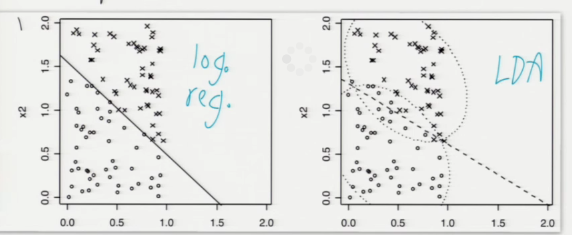
\includegraphics[scale=0.5]{../images/ldavsregression}
							\end{center}
							\item Hence less sensitive to outliers.
							\item Easy and elegant treatment of "partial" class membership; LDA is all-or-nothing.
							\item More robust on some non-gaussian distributions (e.g. large skew).
						\end{itemize}
					\item ROC Curve
						\begin{center}
							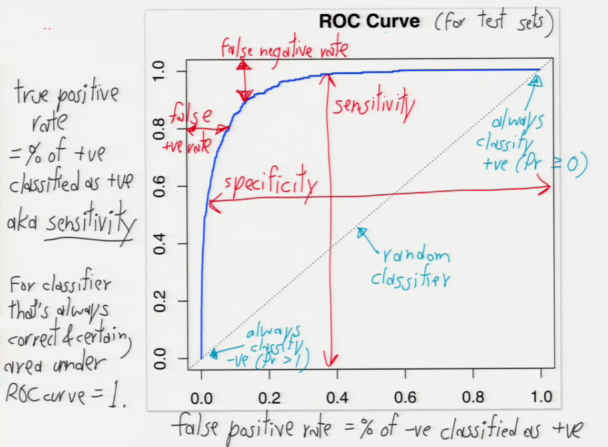
\includegraphics[scale=0.5]{../images/ROCCurve}
						\end{center}
						\begin{itemize}
							\item Receiver Operating Characteristics 
							\item A way of telling you information about the test set, not part of the learning algorithm.
							\item Run classifier on test set, and it shows the rate of false positives vs. true positives for a range of settings.
							\item x-axis false positive rate = \% of negative samples accidentally classified as positive.
							\item y-axis true positive rate = \% of positive that actually got classified as positive (aka sensitivity).
						\end{itemize}
				\end{itemize}
				
		\subsection*{Least-Squares Polynomial Regression}
				\
					\begin{itemize}
						\item Replace each $X_{i}$ with feature vector $\Phi(X_{i})$ with all terms of degree $0 \dots p$.
						\item e.g. $\phi(X_{i}) = \begin{bmatrix}
												X_{i1}^{2} & X_{i1}X_{i2} & X_{i2}^{2} & X_{i1} & X_{i2} & 1 
 											\end{bmatrix}^{T}
 											$
 						\item Can also use non-polynomial features (e.g. edge detectors).
 						\item Otherwise just like linear or logistic regression.
 						\item Logistic regression plus quadratic features = same logistic posteriors as QDA. Very easy to overfit!
							\begin{center}
								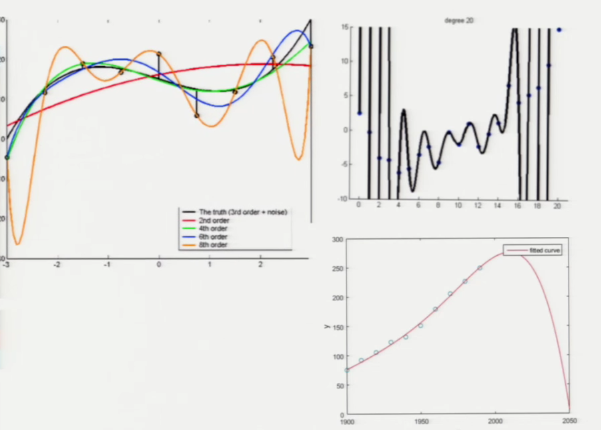
\includegraphics[scale=0.5]{../images/polyregression}
							\end{center}
					\end{itemize}

\end{document}
